\documentclass[11pt]{article}

\usepackage[letterpaper,margin=1in]{geometry}
\usepackage[T1]{fontenc}
\usepackage[utf8]{inputenc}
\usepackage{lmodern}
\usepackage{microtype}
\usepackage{setspace}
\usepackage{amsmath,amssymb,mathtools}
\usepackage{booktabs,longtable,tabularx,array,multirow,threeparttable}
\usepackage{graphicx}
\usepackage{pdflscape}
\usepackage{subcaption}
\usepackage{float}
\usepackage{enumitem}
\usepackage{siunitx}
\usepackage{natbib}
\usepackage{xcolor}
\usepackage{titlesec}
\usepackage{fancyhdr}
\usepackage{appendix}
\usepackage{url}
\usepackage{hyperref}
\usepackage[nameinlink,noabbrev]{cleveref}

% Explicit foreground and background colors are used throughout to prevent
% renderer-dependent contrast failures.
\definecolor{PaperWhite}{HTML}{FFFFFF}
\definecolor{Ink}{HTML}{17212B}
\definecolor{Navy}{HTML}{16324F}
\definecolor{Blue}{HTML}{276FBF}
\definecolor{Teal}{HTML}{1B7F79}
\definecolor{Gold}{HTML}{9A6700}
\definecolor{Red}{HTML}{B42318}
\definecolor{Panel}{HTML}{F2F6FA}
\definecolor{Rule}{HTML}{C7D2DE}
\pagecolor{PaperWhite}
\color{Ink}
\hypersetup{
  colorlinks=true,
  linkcolor=Navy,
  citecolor=Teal,
  urlcolor=Blue,
  pdfborder={0 0 0},
  pdftitle={From Reported Alpha to Reproducible Returns},
  pdfauthor={Sasha Cui}
}
\sisetup{detect-all,group-separator={,},group-minimum-digits=4}
\setstretch{1.08}
\setlength{\parskip}{0.35em}
\setlength{\parindent}{1.2em}
\setlength{\headheight}{22pt}
\setlist{nosep,leftmargin=1.5em}
\newcolumntype{L}[1]{>{\raggedright\arraybackslash}p{#1}}
\titleformat{\section}{\Large\bfseries\color{Navy}}{\thesection}{0.6em}{}
\titleformat{\subsection}{\large\bfseries\color{Navy}}{\thesubsection}{0.6em}{}
\titleformat{\subsubsection}{\normalsize\bfseries\color{Navy}}{\thesubsubsection}{0.6em}{}
\pagestyle{fancy}
\fancyhf{}
\fancyhead[L]{\color{Navy}\small From Reported Alpha to Reproducible Returns}
\fancyhead[R]{\color{Navy}\small Cui}
\fancyfoot[C]{\color{Ink}\thepage}
\renewcommand{\headrulewidth}{0.4pt}
\renewcommand{\headrule}{\hbox to\headwidth{\color{Rule}\leaders\hrule height \headrulewidth\hfill}}

\newcommand{\pct}[1]{\SI{#1}{\percent}}
\newcommand{\bps}[1]{\SI{#1}{\text{bp}}}
\newcommand{\systemname}[1]{\textsf{#1}}
\newcommand{\artifacttier}[1]{\textsf{#1}}
\newcommand{\yes}{\textcolor{Teal}{Yes}}
\newcommand{\no}{\textcolor{Red}{No}}

\InputIfFileExists{generated_results.tex}{}{%
  \PackageError{paper}{generated_results.tex is required}{Run scripts/build_paper_assets.py before compiling.}%
}

\title{\textbf{\color{Navy}From Reported Alpha to Reproducible Returns:}\\
\large A Systematic Artifact Audit of LLM Financial Agents and a Common-Task Test of Mechanism-Inspired Proxies}
\author{Sasha Cui}
\date{August 2026}

\begin{document}
\maketitle

\begin{abstract}
Large-language-model (LLM) financial agents report alpha discovery and trading gains, but their evidence is difficult to compare when artifacts, return streams, timing, costs, and baselines differ. We freeze \SystemCount{} named lineages through 2 August 2026 and audit the \MethodSystemCount{} formula-discovery or trading systems in the primary denominator. Only \ArtifactCountFT{} list a public artifact (\ArtifactRateFT{}; Wilson 95\% CI \ArtifactWilsonFT{}), \NativeDatedOutputCount{} ship any dated native output, and \NativeReturnCount{} provide a monthly return stream compatible with the specified six-country task. This is an availability result, not a zero-return imputation. Separately, we test \ProxyCount{} frozen mechanism-inspired characteristic portfolios in six G7 ex-U.S. markets over \RegressionMonthCount{} common months (\RegressionStartMonth{}--\RegressionEndMonth{}), net of \bps{10} one-way costs. After a disclosed post-outcome correctness repair and subsequent post-runtime limited-liability amendment, \ValidProxyCount{} paths are executable; \PathFailureCandidateCount{} candidates generate \PathFailureEventCount{} country-level failure events and enter Holm and false-discovery accounting with $p=1$. Among executable paths, median annualized factor alpha is \MedianAlphaPct{}; \NominalPositiveCount{} estimates are nominally positive, \HolmPositiveCount{} survive Holm, \MaxTPositiveCount{} survive paired max-$|t|$ adjustment, and \EconomicConfirmedCount{} have simultaneous lower bounds at or above the prespecified 2-percentage-point threshold. Prespecified HAC-lag and block-length sensitivities leave the conclusion intact. The geographic evidence is amended rather than a pristine holdout, and the proxies omit the linguistic, multimodal, intraday, and live-execution mechanisms central to many agents. The main finding is therefore evidence attrition from reported alpha to auditable returns, not a native agent leaderboard.
\end{abstract}

\noindent\textbf{Keywords:} financial agents; large language models; alpha discovery; reproducibility; common-task evaluation; multiple testing; transaction costs

\noindent\textbf{JEL classification:} C52; C55; G11; G12; G17

\section{Introduction}\label{sec:introduction}

Financial-agent research has moved from prompting a language model for a directional opinion to systems that retrieve data, write factor expressions, debate investment theses, retain episodic memory, call execution tools, and revise portfolios. Formula-mining systems report new signals; sequential agents report Sharpe ratios, cumulative returns, or trading decisions; benchmarks increasingly expose leakage, unstable reasoning, style concentration, and long-horizon deterioration. These contributions are heterogeneous by design. Their empirical claims are therefore not commensurable merely because each reports a number labeled ``alpha'' or ``Sharpe ratio.''

The central object of this study is the path from a reported performance claim to a return series that an independent researcher can evaluate under a fixed protocol. That path can break at several distinct points. A primary record may not link code. A repository may expose prompts or an interface but omit data snapshots, generated signals, portfolio weights, or executable return-producing code. A runnable system may depend on proprietary model endpoints, point-in-time news, credentials, or a market simulator that does not map to a monthly equity panel. Even when a return series is available, its universe, timing, factor controls, and costs may be incompatible with another system. Treating every break as a zero return would be wrong; dropping every break from the denominator would be equally misleading.

We address this measurement problem with four linked but explicitly non-equivalent layers. First, we construct a frozen, deduplicated census of \SystemCount{} named system lineages through 2 August 2026. Second, we audit artifacts for the \MethodSystemCount{} formula-discovery and sequential-trading systems that form the main method denominator. Third, we record whether the public materials yield a native return stream that can enter the specified common task without substituting our economic mechanism for the authors' system. Fourth, because native coverage is sparse, we conduct a separate mechanism-inspired transfer exercise using \ProxyCount{} formulas previously encoded from public descriptions. The proxy exercise asks whether characteristic mechanisms associated with the literature survive a uniform international evaluator; it does not reproduce the agents and cannot test their live, linguistic, multimodal, or interactive components.

The design answers three questions. \emph{Availability}: what fraction of named systems provides an identifiable public artifact, license, revision pin, and auditable return-producing path? \emph{Fidelity}: how far can an independent evaluator proceed before a missing component changes the estimand? \emph{Economic transfer}: among frozen mechanism-inspired proxies, what survives geographic transfer, factor adjustment, realized turnover, transaction costs, and simultaneous inference? These questions are intentionally narrower than ``Do LLM agents beat the market?'' A negative availability finding is not a negative return. A failed port is not a failed native strategy. A successful proxy is not evidence that an agent generated deployable alpha.

Four contributions follow. First, the census separates 29 formula-discovery systems, 38 sequential trading or portfolio systems, 23 benchmarks and audits, five community systems, and eight mechanistic comparators. This prevents benchmark platforms and repository-only demonstrations from inflating the method denominator. Second, the artifact ledger preserves every system in its original denominator and reports unavailable artifacts, dependency failures, missing data, incompatible domains, and absent return paths as distinct outcomes with Wilson intervals. Third, the common-task evaluator records signed target weights and post-return drift, charges costs to realized traded notional, uses a parsimonious characteristic-factor benchmark, and applies both conventional and resampling-based multiplicity controls. Fourth, the paper joins each generated headline statistic to immutable input hashes, a producing script, an exact source filter, and a table or figure, so that a reviewer can distinguish frozen evidence from interpretation.

The empirical conclusion is deliberately calibrated. Public artifacts are too sparse and too heterogeneous to support a broad native ranking of the current literature. The international proxy experiment yields \ResultHeadline{}. That finding bears on the transferability of the encoded characteristic mechanisms, not on systems whose claimed edge arises from news interpretation, high-frequency routing, proprietary data, or adaptive model interaction. The strongest result is therefore an evidence-architecture result: the literature has many reported outcomes, substantially fewer public artifacts, and fewer still common-task native returns.

\section{What Is Being Replicated?}\label{sec:estimands}

\subsection{Four objects that must not be conflated}

We use ``replication'' only when the public implementation, model logic, inputs, portfolio rule, and reported evaluation target can be rerun with no economically material substitution. A \emph{native common-task evaluation} retains the system's generated signals or weights but applies a shared return evaluator. A \emph{port} reimplements the authors' explicit rule on compatible data, with every substitution disclosed. A \emph{mechanism-inspired proxy} translates a narrative idea into available characteristics and is evidence only about that translation. The present common-task experiment belongs to the last category. Earlier exploratory files used the word ``replication'' more loosely; this paper and its released ledgers correct that terminology.

This distinction changes both numerator and denominator. If a system requires point-in-time news and the public artifact omits the news snapshot, a price-characteristic substitute cannot be counted as the native system. If source code generates a formula but does not ship the formula selected in the paper, rerunning a hand-picked formula does not recover the paper's stochastic search outcome. If a repository provides a user interface but no portfolio holdings or backtest engine, its presence establishes public inspectability, not return reproducibility.

\subsection{Evidence ladder and failure semantics}

The artifact audit uses an observable four-level ladder:

\begin{description}[style=nextline,leftmargin=1.6em]
  \item[\artifacttier{R0}: no reachable public artifact path.] The frozen primary record does not list an artifact, the listed target is definitively unavailable, or reachability cannot be established at audit time; these states remain separate failure categories.
  \item[\artifacttier{R1}: descriptive or incomplete artifact.] A reachable project page, prompts, pseudocode, screenshots, documentation, or statically incomplete repository exists, but the packaged materials do not expose both source code and a dependency manifest.
  \item[\artifacttier{R2}: packaged executable components.] Observable source code and a dependency or setup manifest are public, but a runner and tests, examples, or configuration support are not all statically observed.
  \item[\artifacttier{R3}: packaged runnable structure.] R2 evidence is accompanied by a visible runner and tests, examples, or configuration support. This is a static packaging classification, not evidence that the native system executed successfully or produced a dated return stream.
\end{description}

Failure labels are observations rather than imputations. ``No public artifact,'' ``unreachable at audit time,'' ``license absent,'' ``environment failure,'' ``required private input,'' ``domain incompatible,'' and ``no dated return path'' remain separate. None is assigned a zero return. Conversely, systems do not disappear from the public-availability denominator because an execution attempt fails.

\section{Literature Census and Evidence Base}\label{sec:census}

\InputIfFileExists{related_literature.tex}{}{%
  \PackageError{paper}{related_literature.tex is required}{The census section has not been generated.}%
}

\subsection{Primary records, versions, and named lineages}

The unit of observation is a named system lineage, not a PDF, repository, benchmark run, or arXiv version. Conference and preprint manifestations are merged. A successor remains within a lineage when it is explicitly presented as a versioned release of the same system and becomes a new row when its architecture and claimed method are distinct. Generic name collisions are resolved by authors, task, and architecture. Benchmarks that evaluate many agents are not counted as candidate methods. The registry preserves all aliases and the rationale for every merge or exclusion.

The initial materials contained 73 raw paper and code links. Normalization yielded 55 seed lineages after resolving a discovery-only list into primary records and merging duplicate Alpha-GPT manifestations. The updated search added 48 lineages and merged one validation study into the existing MarketSenseAI lineage. The frozen total is \SystemCount{}. A PRISMA-like flow is shown in \cref{fig:funnel}; the full registry, including URLs and deduplication notes, appears in \cref{app:registry}. We use PRISMA as a reporting discipline rather than claim that a fast-moving computer-science preprint census can achieve the closure of a clinical systematic review \citep{PageEtAl2021PRISMA}.

\begin{figure}[H]
  \centering
  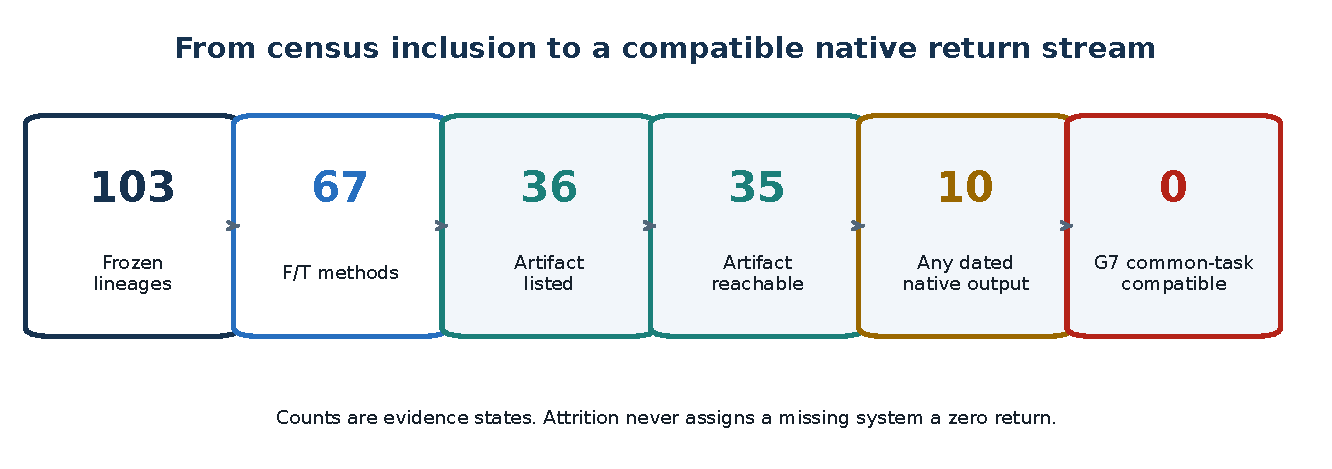
\includegraphics[width=0.94\linewidth]{figures/census_funnel.pdf}
  \caption{Census construction and empirical attrition. Counts are lineages, not publications. The artifact and native-return stages retain the \MethodSystemCount{} formula-discovery and sequential-trading systems as their denominator. A missing artifact or return path is reported as unavailable evidence, never as a zero return.}
  \label{fig:funnel}
\end{figure}

\section{Artifact Audit}\label{sec:artifacts}

\subsection{Observable fields and reproducible checks}

For every registry row, the audit records the primary record, official artifact URL as listed by that record, URL type, reachability at the frozen timestamp, repository owner and name, default-branch head commit, visible license, and static evidence tier. Multiple URLs are retained. Git repositories are pinned with \texttt{git ls-remote}; the audit does not infer a license from repository visibility, and ``no license observed'' is not labeled open source. Project pages, hosted demos, model collections, and anonymous review snapshots are recorded as their actual artifact type rather than relabeled as source code.

The static pass searches for environment specifications, executable entry points, data acquisition instructions, dated signals, holdings, realized returns, tests, and licenses. A smoke attempt is made only when its requirements are public and computationally proportionate. We do not create accounts, buy data, reuse undisclosed credentials, contact authors, or silently replace unavailable inputs. The exact audit timestamp and network error are retained, allowing a later census to distinguish a missing artifact at the cutoff from a transient outage.

The audit's purpose is not to reward large repositories. A concise archive containing dated signals and a timing convention can be more reproducible than a complete application whose evaluation data are absent. Likewise, an R3 packaging classification is not a certification of successful execution or point-in-time integrity. The field answers whether a claimed outcome can enter an independent evaluator, after which leakage, execution, and statistical questions begin.

\subsection{Availability and attrition}

Among the \MethodSystemCount{} primary F/T systems, \ArtifactCountFT{} list at least one public artifact and \ReachableArtifactCountFT{} had a reachable artifact at the frozen audit. The listed-artifact rate is \ArtifactRateFT{} (Wilson 95\% CI \ArtifactWilsonFT{}). \LicensedArtifactCountFT{} expose an observed reuse license, and \PinnedRepoCountFT{} could be pinned to a public Git revision. The tier distribution is \ArtifactTierSummaryFT{}. \Cref{tab:artifact-summary} reports every numerator against the unchanged denominator; \cref{fig:artifact} visualizes attrition by system class.

\InputIfFileExists{tables/artifact_summary.tex}{}{\PackageError{paper}{artifact summary missing}{Run the paper asset builder.}}

\begin{figure}[H]
  \centering
  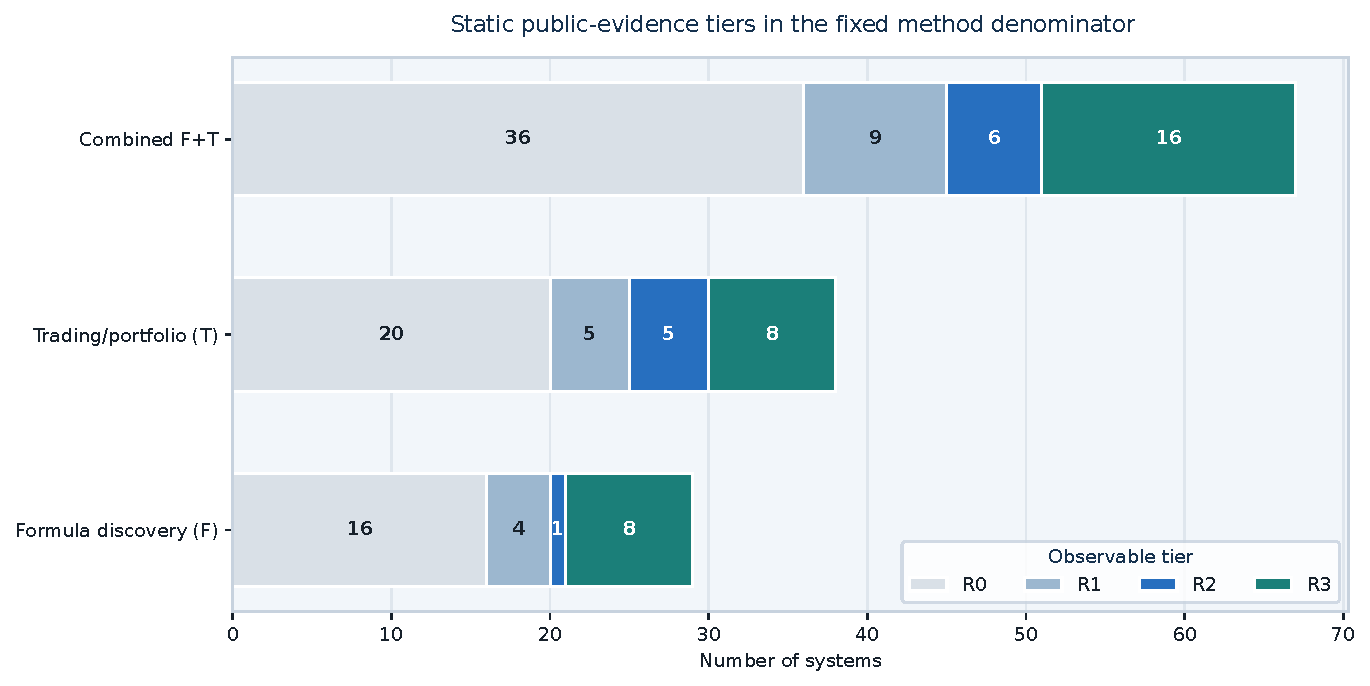
\includegraphics[width=0.96\linewidth]{figures/artifact_attrition.pdf}
  \caption{Public-evidence ladder for the primary method denominator. Colors identify observable evidence tiers, not quality scores. A system can be methodologically strong and still be unavailable for independent common-task evaluation.}
  \label{fig:artifact}
\end{figure}

The public materials yielded \NativeDatedOutputCount{} systems with some shipped dated native output, but \NativeReturnCount{} streams compatible with the specified six-country monthly common task. In the earlier targeted execution audit, \TargetedAuditCount{} artifacts were examined in depth and \TranslatableSeedCount{} supplied one or more ideas that could be translated without claiming a native return reproduction. This distinction reverses a tempting but invalid conclusion: the audit does not observe \MethodSystemCount{} failed strategies; it observes \NativeReturnCount{} directly comparable native return paths and \NativeUnavailableCount{} systems for which the specified native comparison is not identified from public materials.

\section{Common-Task Design}\label{sec:common-task}

\subsection{Protocol locks and geographically external evidence}

The initial confirmatory protocol, candidate formulas, system registry, evaluator, and tests were hashed before any G7 ex-U.S. outcome file was opened. A separate line-level code review conducted after the first run, but before accepting its results, found a future-availability formation filter, an incorrect long--short drift normalization, mismatched country sets, and a mismatch between ordinary and bootstrap calendars. We rejected and archived that run, amended the evaluator, added regression tests and point-estimate/country-count assertions, and created a second lock. The first attempt under that lock then stopped during the Canada build when an extreme gain in a shorted security drove a 100/100 long--short sleeve to nonpositive NAV. A scale audit found no Canadian security total return below -100\%; the failure was a feasible bankruptcy state for the leveraged sleeve, not a percentage-versus-decimal data error. Before another corrected run produced an accepted alpha table or ranking, we froze a limited-liability rule, added path-failure tests, and created the third and current lock. Its SHA-256 is \texttt{\AnalysisLockShort}; both superseded attempts, their hashes, logs, and partial outputs remain in the provenance archive and cannot enter the reported estimates.

The geographically external analysis covers Canada, France, Germany, Italy, Japan, and the United Kingdom from July 1999 through November 2024. Before the initial lock we inspected only file presence, date ranges, row counts, and identifier coverage. U.S. data had already been analyzed during formula development and are therefore labeled retrospective throughout. The first repair followed outcome access and changed the estimation sample and missing-outcome rule; the second followed a runtime path failure and changed failure handling. Both are disclosed protocol deviations. Candidate formulas, signs, markets, costs, thresholds, adjustment procedures, bootstrap seed, and block length did not change. The sample is therefore geographically external and governed by a locked amended evaluator, but it is not described as an untouched or held-out confirmatory test.

The country files come from the international characteristic data maintained by \citet{JensenKellyPedersen2023}. We use the database-provided USD-converted one-month-ahead excess return, USD market-equity weight, total return, and harmonized monthly characteristics. For each country-month, the ex-ante eligible universe is the 1,000 largest securities with a valid identifier and positive formation-date market equity; each candidate then requires its own score inputs. Next-month return availability is never an eligibility or ranking condition. Under Amendment~1, a held security with a missing next-month return receives zero excess return at its frozen ex-ante weight, and the output records gross weight exposed to this convention. A position-adverse sensitivity assigns -100\% to a missing long return and +100\% to a missing short return, so missing exposure contributes minus its absolute weight without future-conditioned reweighting. Missing total returns used for drift remain zero and their exposure is reported separately. All scores, breakpoints, and portfolios are formed within country. For candidates whose full six-country paths remain executable under Amendment~2, a pooled month is retained only when every executable candidate and every control is available in all six countries; candidate returns, turnover, and factors therefore average the identical country set. A failed path does not erase otherwise valid months for executable candidates, but it remains in the original Holm/FDR family of 62 hypotheses with $p=1$. The design avoids mechanical dominance by the largest country. It does not construct local-currency or FX-hedged returns and should not be interpreted as a deployable multicurrency execution study.

\subsection{Frozen proxy family}

The proxy library contains 61 characteristic formulas mapped before the confirmatory analysis from public descriptions in the seed literature, plus one trailing contest sleeve. Candidate formulas combine only information present in the monthly panel: momentum and reversal, volatility and downside risk, valuation, profitability and quality, investment and growth, issuance and leverage, liquidity and turnover, and cross-sectional combinations of those variables. Most formulas are rank sums or differences. The mapping is fully enumerated in \cref{app:candidates}.

The 62 strategies are not agent outputs. They do not invoke an LLM during the geographically external evaluation and do not recreate iterative search, reflection, tool use, news retrieval, images, intraday decisions, human feedback, or live execution. Their value is diagnostic: they hold the return evaluator fixed while asking whether familiar economic mechanisms associated with the papers survive a new geographic domain. This lower-fidelity layer is reported after, and never pooled with, the native artifact audit.

For a cross-sectional score $s_{i,t}$ in country $c$, the main long--short strategy holds the top and bottom country deciles. Each leg is value weighted:
\begin{align}
 w^{+}_{i,t} &= \frac{m_{i,t}}{\sum_{j\in H_{c,t}}m_{j,t}}\mathbf{1}\{i\in H_{c,t}\}, &
 w^{-}_{i,t} &= -\frac{m_{i,t}}{\sum_{j\in L_{c,t}}m_{j,t}}\mathbf{1}\{i\in L_{c,t}\}, \\
 r^{p}_{c,t+1} &= \sum_i \left(w^{+}_{i,t}+w^{-}_{i,t}\right)r^{e}_{i,t+1}.
\end{align}
Long--short portfolios therefore have unit long and unit short exposure. The few long-only rules have unit gross exposure. Each decile side contains at least 20 securities; the top-five exception requires an eligible universe of at least 20 but holds five. Exact side counts and an identifier-based tie-break keep the legs disjoint even when scores tie. The contest proxy selects, using only prior returns, the eligible sleeve with the highest trailing Sharpe over at most 36 months and at least 24 observations.

\subsection{Turnover and trading costs}

Target weights are not differenced against stale targets. If the previous risky-asset weights are $w_{i,t-1}$, the realized USD total security returns are $R_{i,t}$, and the strategy total return is $R^p_t=\sum_iw_{i,t-1}R_{i,t}$, all risky holdings are expressed relative to the same post-return NAV whenever $R^p_t>-1$:
\begin{equation}
  \widetilde w_{i,t}=\frac{w_{i,t-1}(1+R_{i,t})}{1+R^p_t}.
\end{equation}
This retains drift in long and short gross exposures, so their restoration is charged as a trade. If $w_{i,t}^{*}$ is the new target, realized traded notional per dollar of strategy capital is
\begin{equation}
  \tau_t = \sum_i \left|w_{i,t}^{*}-\widetilde w_{i,t}\right|.
\end{equation}
Amendment~2 treats $R^p_t\leq -1$ as a complete-path implementation failure for a candidate or for the trailing-selection contest sleeve. The evaluator never clips the return, restarts the strategy, or injects capital. It writes the failure month, market, realized total return, observed gross strategy return, traded notional, and selected sleeve when applicable. Failure in any included market makes that candidate's pooled path unavailable; country and leave-one-country-out analyses reassess failure using only their included markets. Such a candidate is not assigned a zero return and does not enter regressions. It remains in the prespecified 62-hypothesis family with $p=1$ for Holm and FDR accounting; the bootstrap maximum-statistic procedures are defined over the 27 estimable paths.

The initial establishment of a portfolio is charged at its gross exposure. Net return at one-way cost $c$ basis points is
\begin{equation}
  r^{\mathrm{net}}_{t+1}(c)=r^{p}_{t+1}-\frac{c}{10{,}000}\tau_t.
\end{equation}
The prespecified primary cost is \bps{10}; sensitivity points are 0, 5, 25, and 50 basis points. This transparent linear schedule excludes nonlinear market impact, borrow fees, locate failures, taxes, and currency conversion. It likely understates costs for difficult names and is not a claim of realistic institutional capacity \citep{NovyMarxVelikov2016}.

\subsection{Factor model and effect sizes}

Within each country we construct a market return and five characteristic factor returns using the same eligible universe and value-weighted extreme deciles: size, book-to-market, asset growth, operating profitability, and 12-to-1 momentum. Country factor sleeves are averaged over the exact same six-country set as candidate sleeves. For candidate $j$, the primary six-factor analogue is
\begin{equation}\label{eq:factor-model}
 r^{\mathrm{net}}_{j,t}=\alpha_j+\boldsymbol{\beta}_j^{\top}\mathbf{f}_t+\varepsilon_{j,t}.
\end{equation}
These are transparent characteristic controls rather than the official traded Fama--French international factors \citep{FamaFrench2015,Carhart1997}. Sign conventions do not affect the fitted span, but they do affect coefficient interpretation; the paper therefore emphasizes the intercept and residual risk rather than individual loadings.

We report annualized alpha $12\widehat\alpha_j$, annualized Sharpe $\sqrt{12}\,\bar r_j/s_j$, and annualized appraisal ratio $\sqrt{12}\,\widehat\alpha_j/s(\widehat\varepsilon_j)$. ``Information ratio'' is avoided because no active benchmark-return series is subtracted. Economic relevance thresholds were fixed before validation: annualized alpha of at least two percentage points, an appraisal-ratio increase of at least 0.25, or a Sharpe increase of at least 0.10. Only the alpha threshold is operational here because the evaluator does not contain a sufficiently specified paired active baseline or overlay. Sharpe and appraisal-ratio levels are descriptive and cannot satisfy the materiality count. Statistical significance alone does not satisfy an economic threshold.

\subsection{Dependence and multiple testing}

Equation~\eqref{eq:factor-model} uses a heteroskedasticity- and autocorrelation-consistent covariance matrix \citep{NeweyWest1987}. The lag is fixed mechanically as
\begin{equation}
 L=\left\lfloor 4\left(T/100\right)^{2/9}\right\rfloor.
\end{equation}
The unadjusted two-sided intercept test is descriptive. The primary family contains all \ProxyCount{} frozen candidates. Every cost-level regression and bootstrap for executable candidates uses the same complete candidate--factor calendar. Under Amendment~1, the 24-month Contest warm-up would have fixed the common family start. Under Amendment~2, however, the Contest sleeve is itself a complete-path failure and therefore no longer enters the executable-candidate calendar. The final common regression sample contains \RegressionMonthCount{} realized months, from \RegressionStartMonth{} through \RegressionEndMonth{}. A complete-path failure is excluded from return estimation but receives $p=1$ for Holm and false-discovery accounting rather than leaving those denominators. We report Holm familywise adjusted $p$-values \citep{Holm1979}, Benjamini--Hochberg and Benjamini--Yekutieli false-discovery adjustments \citep{BenjaminiHochberg1995,BenjaminiYekutieli2001}, and a paired moving-block bootstrap over the executable paths.

The bootstrap samples common six-month circular blocks from the complete candidate--factor calendar, re-estimates every executable alpha on the same draw, and centers each bootstrap alpha on its original estimate. With seed 20260802 and \BootstrapCount{} draws, the maximum absolute studentized statistic over those 27 estimable paths supplies a single-step familywise $p$-value and simultaneous 95\% interval. A one-sided global maximum-$t$ statistic over the same estimable set is reported as a reality-check-inspired diagnostic \citep{White2000RealityCheck,Hansen2005SPA,RomanoWolf2005DataSnooping}. It is not an exact White reality check, SPA test, or Romano--Wolf stepdown procedure. We retain both asymptotic and bootstrap results because finite-sample block choices and fixed studentization are themselves modeling decisions.

\section{Results}\label{sec:results}

\subsection{International proxy performance}

At \bps{10} one-way cost, \ValidProxyCount{} of \ProxyCount{} frozen candidates form a complete pooled return series. The other \PathFailureCandidateCount{} candidates generate \PathFailureEventCount{} country-level limited-liability failure events; they enter Holm and FDR family accounting with $p=1$ but are not converted into zero-return observations. Among executable candidates, the median annualized factor alpha is \MedianAlphaPct{} (interquartile range \AlphaIQRPct{}), and \PositiveAlphaCount{} have positive point estimates. Nominal two-sided HAC tests identify \NominalPositiveCount{} positive-alpha candidates at 5\%. Holm adjustment leaves \HolmPositiveCount{}; the 5\% Benjamini--Hochberg and Benjamini--Yekutieli procedures leave \BHPositiveCount{} and \BYPositiveCount{} positive discoveries, respectively. The paired maximum-$|t|$ adjustment over the \ValidProxyCount{} estimable paths leaves \MaxTPositiveCount{}. The reality-check-style global $p$-value over the same estimable set is \RealityCheckP{}. \EconomicConfirmedCount{} candidates have a simultaneous lower alpha bound at or above the prespecified 2-percentage-point threshold.

\begin{landscape}
\InputIfFileExists{tables/primary_results.tex}{}{\PackageError{paper}{primary results missing}{Run the paper asset builder.}}
\end{landscape}

\Cref{fig:forest} plots every estimable annualized alpha with its individual HAC interval and marks the simultaneous inference result. It is deliberately ordered by point estimate rather than system name, making the spread and familywise threshold visible without presenting the rank as a stable leaderboard. The best point estimate is \BestAlphaPct{} for \BestCandidateName{}, but its familywise-adjusted evidence is \BestAdjustedSummary{}. The worst is \WorstAlphaPct{} for \WorstCandidateName{}. Because the strategies share characteristics and holdings, their test statistics are strongly dependent; the paired bootstrap preserves this cross-candidate dependence.

\begin{figure}[htbp]
  \centering
  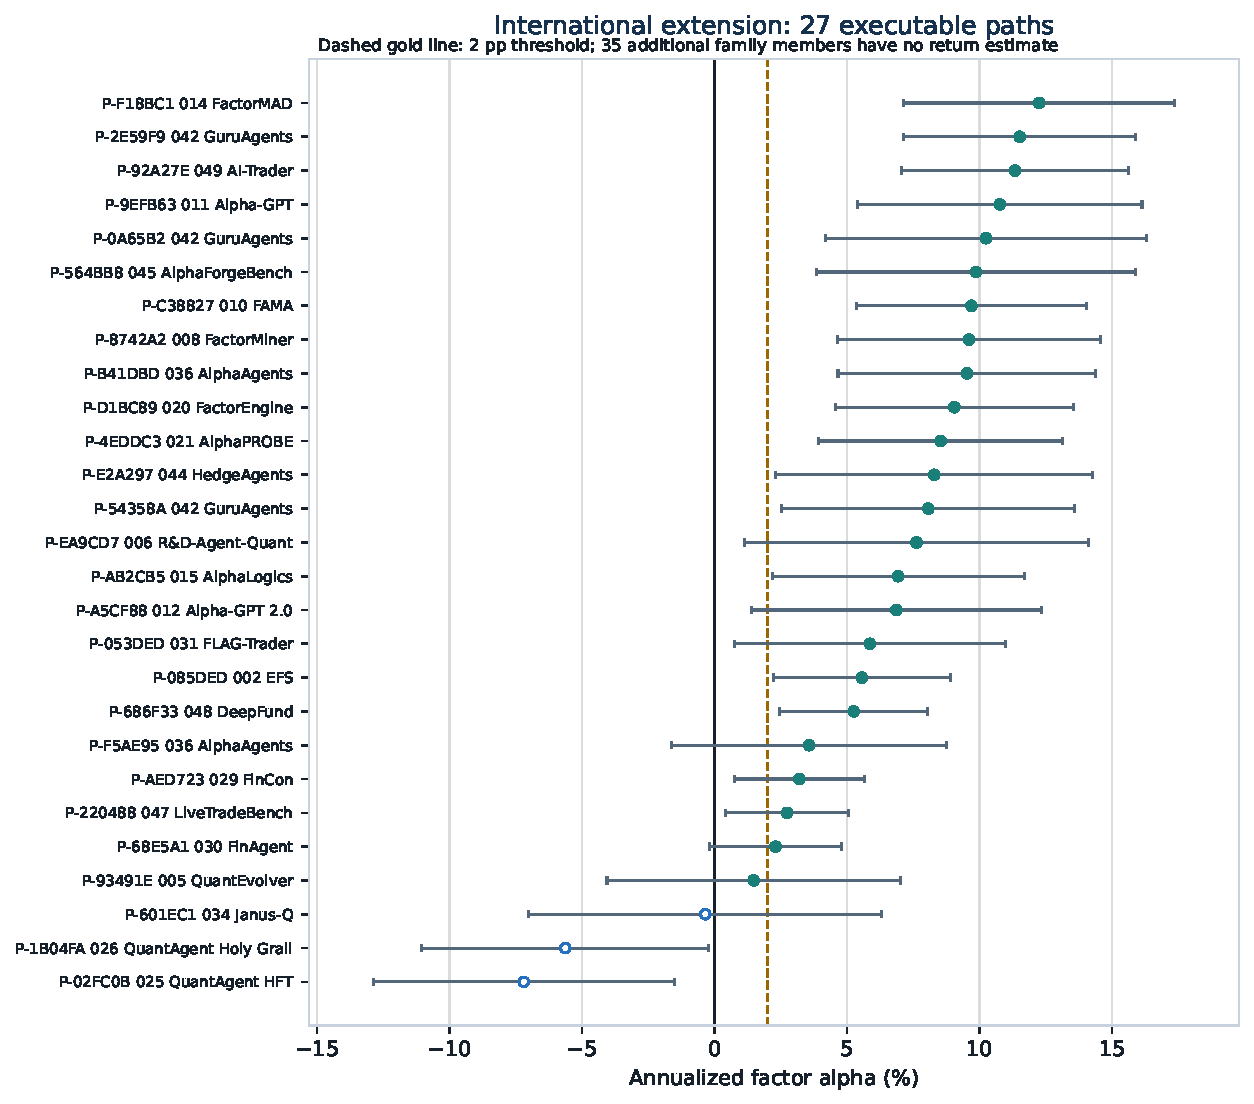
\includegraphics[width=0.98\linewidth]{figures/g7_alpha_forest.pdf}
  \caption{Annualized factor alpha for executable frozen mechanism-inspired proxies, net of \bps{10} one-way costs. The figure omits text-only rows for the complete-path failures, which remain in the 62-hypothesis Holm/FDR families and failure ledger but have no estimated alpha. Thin intervals are individual HAC 95\% intervals; filled markers identify positive estimates. Familywise conclusions over executable paths use the paired maximum-$|t|$ procedure reported in the table, not visual inspection of individual intervals.}
  \label{fig:forest}
\end{figure}

\subsection{Inference-specification robustness}

\HACSensitivitySummary{} \BlockSensitivitySummary{} The prespecified choices therefore change the exact discovery count without changing the qualitative conclusion that a nontrivial subset of executable proxies survives stringent adjustment. \Cref{tab:inference-sensitivity} reports the full count grid and keeps the 62-hypothesis Holm/FDR denominator distinct from the 27-path resampling family.

\InputIfFileExists{tables/inference_sensitivity.tex}{}{\PackageError{paper}{inference sensitivity table missing}{Run the paper asset builder.}}

\subsection{Turnover and cost sensitivity}

The cross-candidate median of each successful path's median monthly traded notional is \MedianTurnover{} per dollar of strategy capital, with a cross-candidate interquartile range of \TurnoverIQR{}. At \bps{10}, the median annualized alpha reduction relative to gross is \MedianCostDragPct{}. \BreakEvenBelowTenCount{} candidates with positive gross alpha have an estimated alpha break-even cost below 10 basis points. At 25 and 50 basis points, the numbers of positive-alpha point estimates fall to \PositiveAtTwentyFive{} and \PositiveAtFifty{}.

\begin{figure}[H]
  \centering
  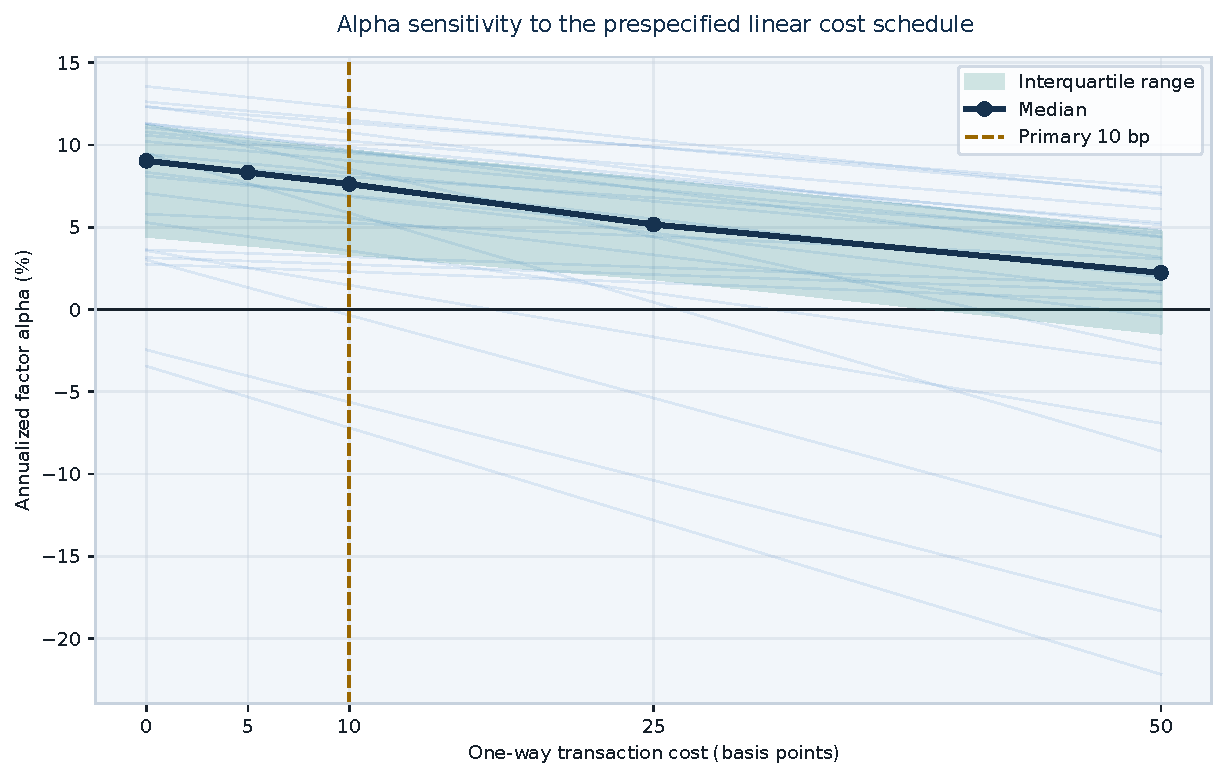
\includegraphics[width=0.95\linewidth]{figures/cost_sensitivity.pdf}
  \caption{Transaction-cost sensitivity. Lines show the cross-candidate distribution of annualized factor alpha at prespecified one-way cost levels. All colors and labels are fixed in the rendering script; the \bps{10} primary point is highlighted.}
  \label{fig:costs}
\end{figure}

Linear cost sensitivity is useful precisely because it reveals which conclusions rely on turnover assumptions. It is not a market-impact model. Strategies concentrated in small or hard-to-borrow securities may incur substantially larger costs, while patient institutional crossing could reduce costs for liquid large-cap portfolios. The top-1,000 filter and value weighting mitigate, but do not remove, this uncertainty.

Missing next-month outcomes are also economically consequential for concentrated rules. Across candidate--country series, median mean missing-excess-return exposure is \MedianMissingExposure{}, the 95th percentile is \MissingExposurePninetyfive{}, and the largest single-month exposure is \MaxMissingExposure{}. Under the position-adverse sensitivity, median alpha is \AdverseMedianAlphaPct{}, \AdverseNominalPositiveCount{} candidates are nominally positive, \AdverseHolmPositiveCount{} survive Holm, and \AdverseEconomicConfirmedCount{} retain a simultaneous lower alpha bound at or above 2 percentage points. The adverse policy also changes the common factor returns, so factor-adjusted alpha need not move monotonically downward even though every missing position receives its portfolio-specific worst-sign return. This sensitivity is intentionally severe and is not a claim about actual delisting returns; it shows how much the primary zero-return convention matters without selecting the investable universe using future coverage.

\subsection{Country dispersion and leave-one-country-out stability}

The pooled result can conceal geographic concentration. The originally generated country and leave-one-out diagnostics allowed each panel's executable set to determine its calendar, so they mixed geographic removal with calendar changes. During submission QA we therefore added a post-hoc diagnostic that holds the \ValidProxyCount{} primary executable candidates and the \RegressionMonthCount{}-month primary calendar fixed for every country and exclusion. This diagnostic does not alter the primary pooled estimates. On that fixed panel, the median number of countries with a positive alpha is \MedianPositiveCountries{} of six. \AllCountryPositiveCount{} of the \ValidProxyCount{} candidates are positive in every country, and \NoCountryPositiveCount{} are positive in none. The most favorable country by median alpha is \BestCountry{}, while the least favorable is \WorstCountry{}. These rankings are descriptive and are not a second multiplicity-adjusted discovery exercise.

Holding all \ValidProxyCount{} candidates and \RegressionMonthCount{} months fixed, the cross-candidate median alpha changes by at most \MaxLeaveOneOutMedianShiftPct{} when one country is removed. For the leading candidate, the leave-one-country-out range is \BestCandidateLooRangePct{}. \Cref{fig:countries} distinguishes widespread transfer from results driven by a single market.

\begin{figure}[H]
  \centering
  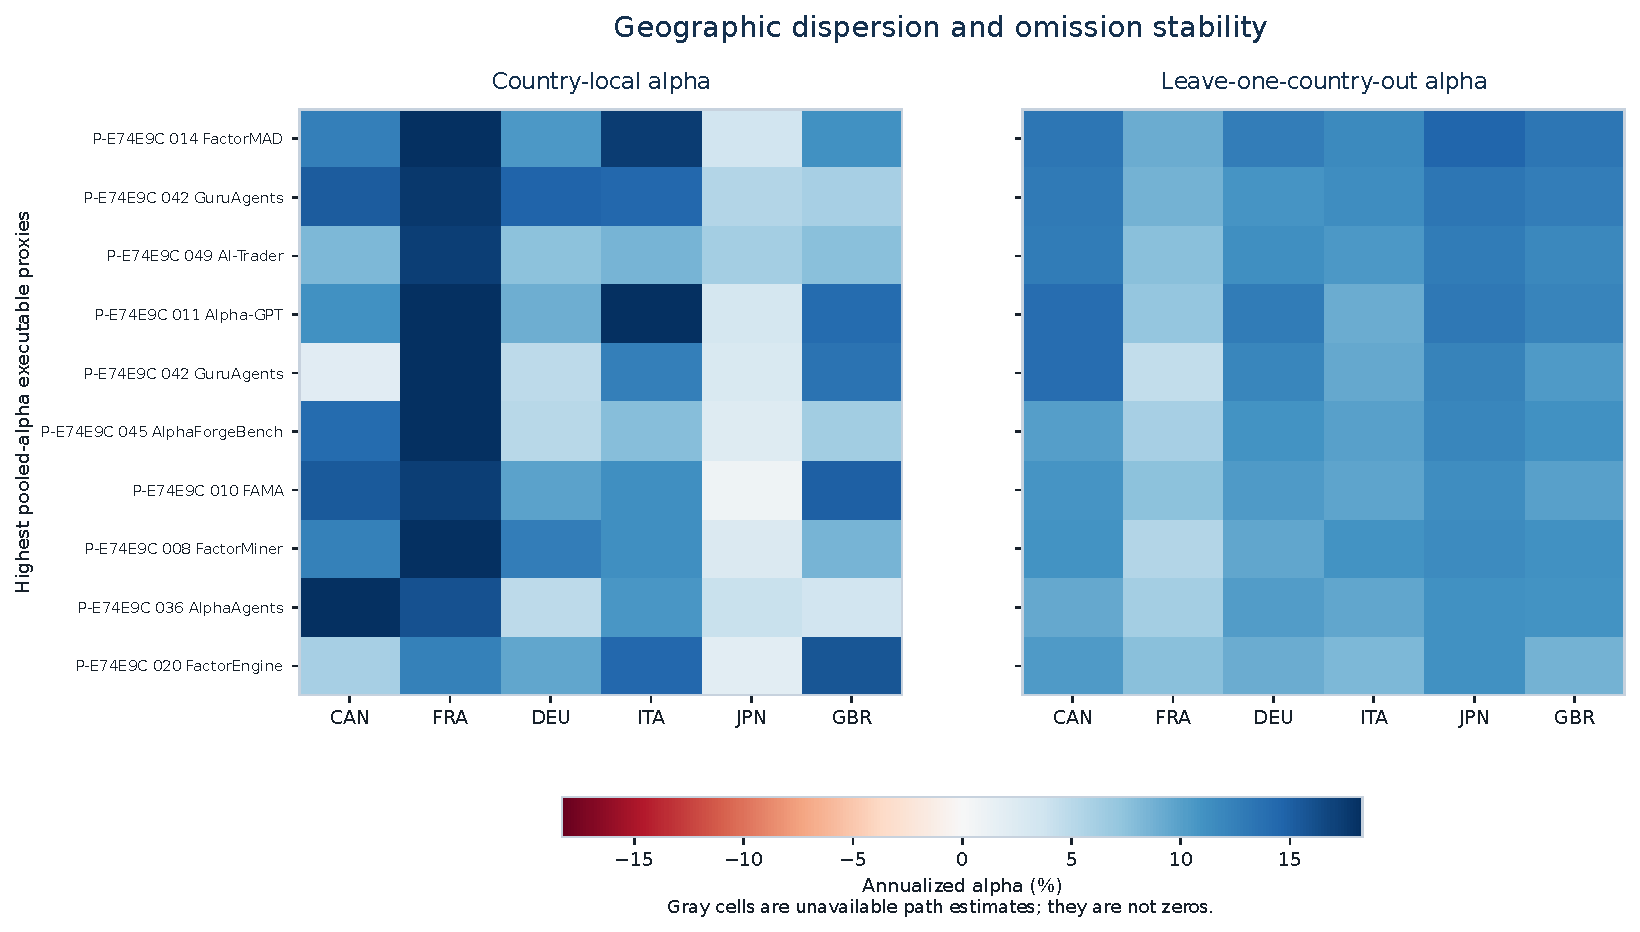
\includegraphics[width=0.96\linewidth]{figures/country_robustness.pdf}
  \caption{Post-hoc fixed-calendar country-level and leave-one-country-out robustness for the highest pooled-alpha proxies. Every cell uses the same \ValidProxyCount{} candidates and \RegressionMonthCount{} months as the primary regression calendar. Country estimates are net of \bps{10} and use country-local characteristic controls. These estimates diagnose heterogeneity; they do not redefine the primary family.}
  \label{fig:countries}
\end{figure}

\subsection{Retrospective U.S. comparison}

The U.S. analysis uses the current amended evaluator, but the U.S. return history informed formula development and is not held out. Its role is to measure transport, not confirmation. To avoid conflating transport with sample length, the displayed comparison re-estimates G7 alpha on the U.S. calendar of August 2001 through December 2024. Among the \JointlyEstimableCount{} jointly estimable proxies, the same-window Spearman correlation is \SameWindowUSGSevenSpearman{} and \SameWindowSignAgreementCount{} have the same alpha sign. Using the full \RegressionMonthCount{}-month primary G7 calendar instead yields correlation \USGSevenSpearman{} and sign agreement \SignAgreementCount{}. Across all 62 executable U.S. paths, \USNominalPositiveCount{} are nominally positive at 5\%; on the shared calendar, \SameWindowGSevenNominalPositiveCount{} of the \ValidProxyCount{} G7 paths are nominally positive. The unequal candidate denominators are reported rather than imputing returns for the \PathFailureCandidateCount{} international path failures. This contrast illustrates why a previously examined market cannot stand in for external validation.

\begin{figure}[H]
  \centering
  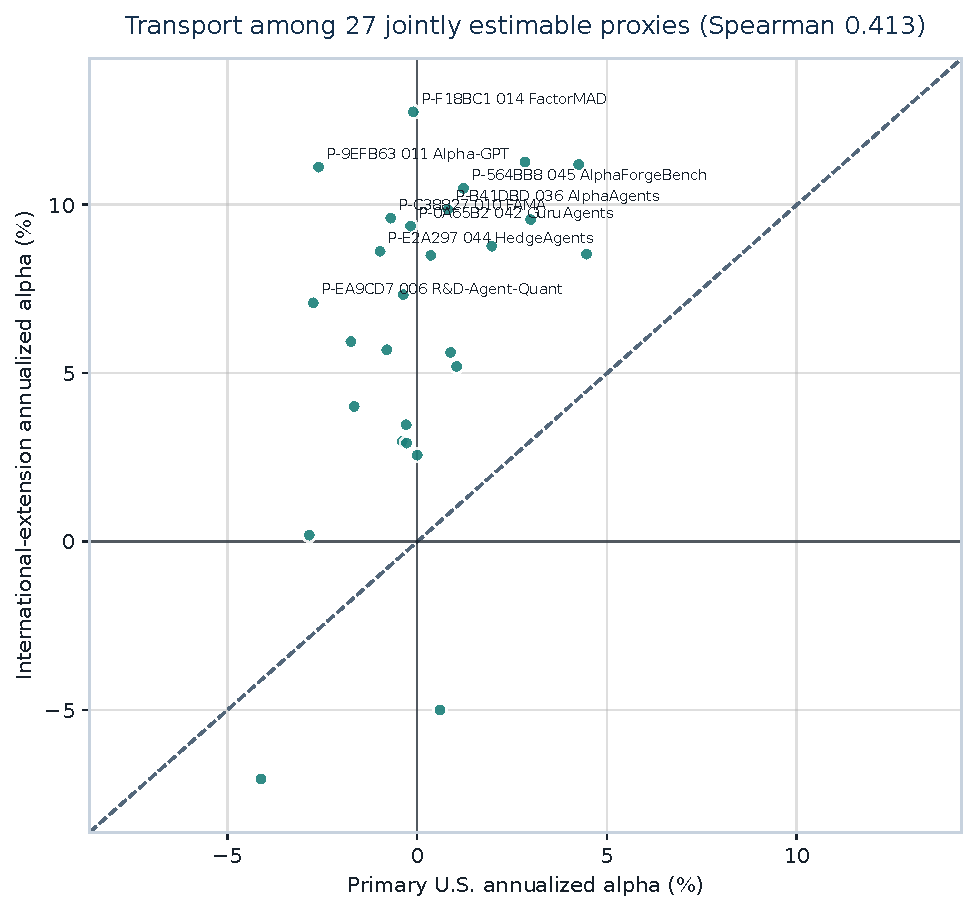
\includegraphics[width=0.82\linewidth]{figures/usa_g7_transfer.pdf}
  \caption{Retrospective U.S. versus geographically external G7 ex-U.S. annualized alpha on the shared August 2001--December 2024 calendar under the current amended evaluator. The diagonal denotes equal performance, not a test threshold. Labels identify large disagreements.}
  \label{fig:transfer}
\end{figure}

\section{Interpretation}\label{sec:interpretation}

\subsection{What the evidence supports}

The artifact census supports a concrete availability claim: \ArtifactRateFT{} of the primary systems linked a public artifact at the cutoff, and fewer exposed a complete dated return path. Because unsuccessful or unavailable systems stay in the denominator, this rate is not inflated by conditioning on what happened to be runnable. The result is substantively important for cumulative science. Without a revision pin, timing convention, generated signal, and portfolio path, independent researchers cannot determine whether a performance difference comes from the model, the data snapshot, the prompt, the portfolio rule, or the evaluator.

The common-task evidence supports a different claim: in a geographically external sample evaluated with the disclosed post-outcome correctness repair and subsequent path-failure amendment, realized turnover, \bps{10} costs, common factor controls, and simultaneous inference yield \ResultInterpretation{}. This is more informative than selecting the best nominal proxy from the already-viewed U.S. sample, but less clean than an untouched validation run. It is also less informative than rerunning native agents because the proxy library deliberately removes many mechanisms that make those agents distinctive.

The two layers reinforce one conclusion without being pooled. Native heterogeneity prevents a broad apples-to-apples ranking; a strict common task is possible only after moving to lower-fidelity characteristic translations. The resulting loss of fidelity is itself evidence about the maturity of the public evaluation infrastructure. A field can have interesting methods and still lack the artifacts needed for comparative empirical accumulation.

\subsection{What the evidence does not support}

The paper does not show that LLMs cannot generate alpha, that every reported result is overstated, or that public code is a sufficient condition for validity. It does not test proprietary deployments. It does not recreate prompt sampling, model-version drift, human oversight, retrieval corpora, textual reasoning, image inputs, market microstructure, or endogenous execution. It cannot attribute proxy performance to an LLM, because no LLM acts during the proxy evaluation. It also does not interpret missing public artifacts as negative returns.

Positive counterexamples matter. A follow-up from the MarketSenseAI research lineage provides unusually explicit external-time validation and limitation discussion, while recent work on macroeconomic-agent investment decisions illustrates how narrower tasks can support more interpretable tests. Independent benchmarks add complementary evidence: FINSABER reports long-horizon deterioration; StockBench finds that most tested agents do not beat buy-and-hold in its setting; KTD-Fin isolates style exposure and memory effects; PortBench shows that many portfolio-profile pairs fail a simple equal-weight comparator; and AlphaQT-Bench separates executable code generation from quantitative reasoning \citep{FatourosMetaxas2026SignalOrNoise,LiEtAl2026FINSABER,ChenEtAl2025StockBench,ZhuEtAl2026KTDFin,ZhaoChenSu2026PortBench,LuoEtAl2026AlphaQT}. These studies do not prove a universal negative. They demonstrate that evaluation choices can dominate a generic ``agent'' label.

\subsection{Design implications for future agent studies}

A high-information release need not publish proprietary model weights or licensed market data. It should publish a revision-pinned evaluation manifest, exact universe and timing rules, immutable signal or position hashes, cost conventions, baseline return series, random seeds, failure counts, and a script that recomputes tables from appropriately licensed inputs. Stochastic agents should report the distribution across runs and model versions, not only the best trajectory. Systems that search many formulas should treat search breadth as multiplicity and preserve the rejected-candidate denominator \citep{HarveyLiuZhu2016}.

Common tasks should separate generation from evaluation. A sealed evaluator can accept dated weights or orders without receiving private prompts or training code. Multiple tracks can preserve domain fidelity: monthly cross-sectional equity, event-driven news, intraday execution, crypto, and endogenous multi-agent simulation should not be collapsed into one score. The common-task framework is useful because it fixes the scoring rule while allowing methods to differ \citep{HellumEtAl2025CommonTask}; it becomes misleading when compatibility is achieved by replacing the method's central mechanism.

\section{Threats to Validity}\label{sec:limitations}

\paragraph{Census closure.} The cutoff is precise, but the literature is unusually fast moving and terminology is unstable. Search queries, citation chaining, benchmark references, and seed repositories reduce omission risk without eliminating it. ArXiv replacements and newly public repositories after the cutoff should be treated as new census waves, not silently backfilled into this denominator.

\paragraph{Public-only observation.} No authors were contacted, in accordance with the frozen execution decision. Some teams may have shareable artifacts that are not linked publicly; the audit measures public reproducibility at the cutoff, not willingness to collaborate privately. Network reachability is timestamped because an outage and a missing link are different observations.

\paragraph{Static fidelity classification.} File signatures can establish the presence of code, environments, outputs, and licenses, but not semantic correctness. A smoke test can fail because of platform drift rather than a scientific defect. For that reason, execution failures are categorized and the static tier is not called a quality score.

\paragraph{Proxy validity.} Translating a paper description to JKP characteristics involves judgment. The formulas capture recognizable economic motifs, not the full systems. They may omit the very information on which the reported edge depends. The proxy results therefore have construct validity for characteristic transfer and limited validity for agent performance.

\paragraph{Validation interpretation.} The analyst did not examine G7 ex-U.S. outcomes until after the initial lock, but Amendment~1 followed the first run and changed the missing-outcome and common-sample rules. The first attempt under that amendment then exposed a nonpositive-NAV path before producing an accepted corrected alpha table, prompting Amendment~2's limited-liability rule and a third lock. Both superseded attempts are archived and excluded. This is geographically external evidence under a transparent post-outcome correctness repair and post-runtime path rule, not a pristine confirmatory holdout. The literature and underlying characteristics are globally known, so the design also does not claim that every formula was historically unknown or that the data are live-forward. The U.S. analysis is explicitly retrospective.

\paragraph{Limited liability and path dependence.} A 100/100 long--short portfolio can lose more than its starting NAV when a shorted security rises sufficiently. Treating that event as a missing observation, clipping it to -100\%, or restarting with new capital would change the strategy. The amended evaluator instead records complete-path failure, preserves the original 62-hypothesis Holm/FDR denominator with $p=1$, and estimates returns only for executable paths. The originally generated country and leave-one-out files consequently had different executable sets and calendars; the paper reports the separately labeled fixed-candidate, fixed-calendar diagnostic to remove that ambiguity.

\paragraph{Return measurement.} Monthly top-1,000 portfolios cannot evaluate high-frequency, event-driven, crypto, derivative, or market-making systems. Database-provided returns may embed delisting, currency, and investability conventions that differ from a trading desk. Equal country weights answer a transfer question but do not describe a market-cap-weighted global mandate.

\paragraph{Costs and constraints.} Linear traded-notional costs omit price impact, financing, borrow constraints, taxes, and operational latency. Weight concentration and turnover diagnostics expose some implementation risk but do not establish capacity. Long--short gross exposure is normalized rather than optimized.

\paragraph{Inference.} HAC inference depends on lag choice, and the moving-block bootstrap depends on block length and fixed studentization. Sixty-two correlated candidates make nominal order statistics unstable. We therefore report effect sizes, individual intervals, Holm, FDR, simultaneous bootstrap intervals, and the complete family rather than one preferred $p$-value. The single-step maximum statistic is not represented as a stepdown procedure.

\section{Reproducibility, Licensing, and Responsible Use}\label{sec:reproducibility}

The release separates source code, original metadata, generated summaries, and third-party references. Project code is licensed under Apache License 2.0; the paper, protocols, and original registry annotations are licensed under Creative Commons Attribution 4.0. Third-party papers, repositories, and market data retain their own terms and are not relicensed or redistributed. The artifact ledger records observed upstream licenses but does not interpret legal compatibility. Generated return files derived from restricted source data remain on the authorized research system and are represented in the public provenance layer by hashes and aggregate tables where redistribution is not permitted.

The current amended lock covers the immutable protocol and both amendments, decision record, source link lists, 103-lineage registry, 62-candidate registry, evaluator, formulas, and unit tests. The locked protocol's released SHA-256 remains \texttt{0a0515cedbb2\ldots}; later implementation-wording clarifications and the post-hoc fixed-calendar diagnostic are isolated in \texttt{docs/reporting\_addendum.md} rather than silently changing that file. The analysis and diagnostic manifests record host-independent paths, package versions, dates, seeds, and input/output hashes. The owner review packet maps each headline claim to a CSV row and marks factual, statistical, citation, license, and visual checks separately. Owner approval remains pending until the named author reviews this draft.

No human participants or private personal data are used. No author was contacted and no orders were transmitted. Results are retrospective research evidence, not investment advice. The code includes no automated brokerage connection. Users who adapt the evaluator bear responsibility for data licenses, market rules, model governance, and trading risk.

\paragraph{AI assistance disclosure.} The author used OpenAI Codex and documented language-model tools for literature organization, code assistance, diagnostic review, and prose editing. Model-assisted work did not determine authorship. The author is responsible for verifying citations, inclusion decisions, statistical specifications, results, and claims before submission. Substantive formula mappings, analysis decisions, and human-review status are preserved in the project records.

\section{Conclusion}\label{sec:conclusion}

This study replaces an underspecified contest over reported Sharpe ratios with an auditable sequence from claim to artifact to return. The frozen census contains \SystemCount{} system lineages, of which \MethodSystemCount{} are primary formula-discovery or sequential-trading methods. Public artifact and native-return coverage fall sharply along the evidence ladder. A separately labeled library of \ProxyCount{} mechanism-inspired characteristic strategies permits a stringent international common-task test, but not a native agent ranking. Under the current amended evaluator and its disclosed path-failure rule, \ConclusionResult{}.

The practical implication is constructive. Stronger evidence does not require every project to expose a production stack. It requires preserving the empirical object that connects a method to a claim: dated signals or weights, timing, universe, evaluator, costs, baselines, search denominator, and versioned code. With those pieces, heterogeneous agents can be compared in compatible tracks and updated evidence can accumulate. Without them, the distance from reported alpha to reproducible returns remains the dominant result.

\clearpage
\begin{appendices}

\section{Frozen System Registry}\label{app:registry}

\begin{landscape}
\InputIfFileExists{tables/system_registry.tex}{}{\PackageError{paper}{system registry table missing}{Run the paper asset builder.}}
\end{landscape}

\section{Frozen Proxy Registry}\label{app:candidates}

\begin{landscape}
\InputIfFileExists{tables/candidate_registry.tex}{}{\PackageError{paper}{candidate registry table missing}{Run the paper asset builder.}}
\end{landscape}

\section{Artifact Failure Ledger}\label{app:failures}

\begin{landscape}
\InputIfFileExists{tables/artifact_failures.tex}{}{\PackageError{paper}{artifact failure table missing}{Run the paper asset builder.}}
\end{landscape}

This table concerns failures in retrieving or executing public artifacts. The amended evaluator records limited-liability events separately in \texttt{candidate\_path\_failures.csv}. Those events are implementation path states, not artifact failures or zero returns.

\section{Limited-Liability Path Failures}\label{app:path-failures}

\begin{landscape}
\InputIfFileExists{tables/path_failures.tex}{}{\PackageError{paper}{path failure table missing}{Run the paper asset builder.}}
\end{landscape}

\section{Protocol, Estimands, and Deviations}\label{app:protocol}

The primary estimand is the intercept in \cref{eq:factor-model} for an equal-country G7 ex-U.S. sleeve, net of \bps{10} one-way costs. The constructor grid uses formation months July 1999--November 2024 and realized-return months August 1999--December 2024; after executable-candidate common-calendar formation, the final regression sample contains \RegressionMonthCount{} months from \RegressionStartMonth{} through \RegressionEndMonth{}. The family contains 62 frozen proxies; complete-path failures have no return estimand but enter Holm and FDR accounting with $p=1$. The minimum planned bootstrap count was 2,000, with 10,000 preferred if compute permitted; the executed count is \BootstrapCount{}. The frozen random seed is 20260802 and the circular block length is six months. \ProtocolDeviationStatement{}

The fixed-calendar country and leave-one-country-out diagnostic was added post hoc during submission QA after we observed that the originally generated descriptive panels allowed country-specific executable sets to induce unequal estimation windows. The diagnostic holds the \ValidProxyCount{} primary executable candidates and their \RegressionMonthCount{}-month calendar fixed, reruns country-local factor regressions, and removes one country at a time without changing candidate membership or dates. Its script, inputs, output, and manifest are separately hashed. It is a robustness diagnostic, not a new confirmatory endpoint.

The artifact estimand is a public-evidence proportion at the cutoff. Its denominator is fixed by registry inclusion, and its confidence interval is Wilson's score interval. Native execution, translated ports, and mechanism-inspired proxies are never combined in one performance numerator.

\section{Additional Robustness Tables}\label{app:robustness}

\begin{landscape}
\InputIfFileExists{tables/cost_results.tex}{}{\PackageError{paper}{cost table missing}{Run the paper asset builder.}}

\InputIfFileExists{tables/country_results.tex}{}{\PackageError{paper}{country table missing}{Run the paper asset builder.}}
\end{landscape}

\section{Claim-to-Output Map}\label{app:claims}

\begin{landscape}
\InputIfFileExists{tables/claim_map.tex}{}{\PackageError{paper}{claim map missing}{Run the paper asset builder.}}
\end{landscape}

\end{appendices}

\clearpage
\bibliographystyle{apalike}
\bibliography{references}

\end{document}
